
% Template for Elsevier CRC journal article
% version 1.2 dated 09 May 2011

% This file (c) 2009-2011 Elsevier Ltd.  Modifications may be freely made,
% provided the edited file is saved under a different name

% This file contains modifications for Procedia Computer Science
% but may easily be adapted to other journals

% Changes since version 1.1
% - added "procedia" option compliant with ecrc.sty version 1.2a
%   (makes the layout approximately the same as the Word CRC template)
% - added example for generating copyright line in abstract

%-----------------------------------------------------------------------------------

%% This template uses the elsarticle.cls document class and the extension package ecrc.sty
%% For full documentation on usage of elsarticle.cls, consult the documentation "elsdoc.pdf"
%% Further resources available at http://www.elsevier.com/latex

%-----------------------------------------------------------------------------------

%%%%%%%%%%%%%%%%%%%%%%%%%%%%%%%%%%%%%%%%%%%%%%%%%%%%%%%%%%%%%%
%%%%%%%%%%%%%%%%%%%%%%%%%%%%%%%%%%%%%%%%%%%%%%%%%%%%%%%%%%%%%%
%%                                                          %%
%% Important note on usage                                  %%
%% -----------------------                                  %%
%% This file should normally be compiled with PDFLaTeX      %%
%% Using standard LaTeX should work but may produce clashes %%
%%                                                          %%
%%%%%%%%%%%%%%%%%%%%%%%%%%%%%%%%%%%%%%%%%%%%%%%%%%%%%%%%%%%%%%
%%%%%%%%%%%%%%%%%%%%%%%%%%%%%%%%%%%%%%%%%%%%%%%%%%%%%%%%%%%%%%

%% The '3p' and 'times' class options of elsarticle are used for Elsevier CRC
%% Add the 'procedia' option to approximate to the Word template
%\documentclass[3p,times,procedia]{elsarticle}
\documentclass[3p,times]{elsarticle}

%% The `ecrc' package must be called to make the CRC functionality available
\usepackage{ecrc}
\usepackage[utf8]{inputenc}
\usepackage{listings}


\usepackage{bigfoot}
\usepackage{hyperref}
\usepackage{graphicx}
\graphicspath{ {./images/} }
%% The ecrc package defines commands needed for running heads and logos.
%% For running heads, you can set the journal name, the volume, the starting page and the authors

%% set the volume if you know. Otherwise `00'
\volume{00}

%% set the starting page if not 1
\firstpage{1}

%% Give the name of the journal
\journalname{Procedia Computer Science}

%% Give the author list to appear in the running head
%% Example \runauth{C.V. Radhakrishnan et al.}
\runauth{}

%% The choice of journal logo is determined by the \jid and \jnltitlelogo commands.
%% A user-supplied logo with the name <\jid>logo.pdf will be inserted if present.
%% e.g. if \jid{yspmi} the system will look for a file yspmilogo.pdf
%% Otherwise the content of \jnltitlelogo will be set between horizontal lines as a default logo

%% Give the abbreviation of the Journal.  Contact the journal editorial office if in any doubt
\jid{procs}

%% Give a short journal name for the dummy logo (if needed)
\jnltitlelogo{Procedia Computer Science}

%% Provide the copyright line to appear in the abstract
%% Usage:
%   \CopyrightLine[<text-before-year>]{<year>}{<restt-of-the-copyright-text>}
%   \CopyrightLine[Crown copyright]{2011}{Published by Elsevier Ltd.}
%   \CopyrightLine{2011}{Elsevier Ltd. All rights reserved}
\CopyrightLine{2011}{Published by Elsevier Ltd.}

%% Hereafter the template follows `elsarticle'.
%% For more details see the existing template files elsarticle-template-harv.tex and elsarticle-template-num.tex.

%% Elsevier CRC generally uses a numbered reference style
%% For this, the conventions of elsarticle-template-num.tex should be followed (included below)
%% If using BibTeX, use the style file elsarticle-num.bst

%% End of ecrc-specific commands
%%%%%%%%%%%%%%%%%%%%%%%%%%%%%%%%%%%%%%%%%%%%%%%%%%%%%%%%%%%%%%%%%%%%%%%%%%

%% The amssymb package provides various useful mathematical symbols
\usepackage{amssymb}
%% The amsthm package provides extended theorem environments
%% \usepackage{amsthm}

%% The lineno packages adds line numbers. Start line numbering with
%% \begin{linenumbers}, end it with \end{linenumbers}. Or switch it on
%% for the whole article with \linenumbers after \end{frontmatter}.
%% \usepackage{lineno}

%% natbib.sty is loaded by default. However, natbib options can be
%% provided with \biboptions{...} command. Following options are
%% valid:

%%   round  -  round parentheses are used (default)
%%   square -  square brackets are used   [option]
%%   curly  -  curly braces are used      {option}
%%   angle  -  angle brackets are used    <option>
%%   semicolon  -  multiple citations separated by semi-colon
%%   colon  - same as semicolon, an earlier confusion
%%   comma  -  separated by comma
%%   numbers-  selects numerical citations
%%   super  -  numerical citations as superscripts
%%   sort   -  sorts multiple citations according to order in ref. list
%%   sort&compress   -  like sort, but also compresses numerical citations
%%   compress - compresses without sorting
%%
%% \biboptions{comma,round}

% \biboptions{}

% if you have landscape tables
\usepackage[figuresright]{rotating}

% put your own definitions here:
%   \newcommand{\cZ}{\cal{Z}}
%   \newtheorem{def}{Definition}[section]
%   ...

% add words to TeX's hyphenation exception list
%\hyphenation{author another created financial paper re-commend-ed Post-Script}

% declarations for front matter

\begin{document}

\begin{frontmatter}

%% Title, authors and addresses

%% use the tnoteref command within \title for footnotes;
%% use the tnotetext command for the associated footnote;
%% use the fnref command within \author or \address for footnotes;
%% use the fntext command for the associated footnote;
%% use the corref command within \author for corresponding author footnotes;
%% use the cortext command for the associated footnote;
%% use the ead command for the email address,
%% and the form \ead[url] for the home page:
%%
%% \title{Title\tnoteref{label1}}
%% \tnotetext[label1]{}
%% \author{Name\corref{cor1}\fnref{label2}}
%% \ead{email address}
%% \ead[url]{home page}
%% \fntext[label2]{}
%% \cortext[cor1]{}
%% \address{Address\fnref{label3}}
%% \fntext[label3]{}

\dochead{}
%% Use \dochead if there is an article header, e.g. \dochead{Short communication}
%% \dochead can also be used to include a conference title, if directed by the editors
%% e.g. \dochead{17th International Conference on Dynamical Processes in Excited States of Solids}

\title{Android mempry forensics}

%% use optional labels to link authors explicitly to addresses:
%% \author[label1,label2]{<author name>}
%% \address[label1]{<address>}
%% \address[label2]{<address>}

\author{}

\address{}

\begin{abstract}
Smart phones today are getting ever more powerful, and capable of doing most of the tasks usually associated 
with computers. This have made them increasingly interesting in forensics investigations and information 
theft. In this paper we present the findings we have done when looking at the volatile memory of a virtual 
Android device. In our research we have used string search, hex editor and other tools to search through the memory to 
find cleartext information to prove what sort of information that are stored here. %Prove? skal vi bevise noe? "See what information we could find elns"
We also discuss the 
possibility and usefulness of automated forensics tools to look through smart phone memory and the 
difficulties faced when developing such tools. Another aspect of our research was to look at secure applications 
to see whether or not the volatile memory is taken into account in development. This research provides a 
baseline for further development of memory analysis tools, proving its usefulness and what information  you 
can expect to find on the subject. 
\end{abstract}

\begin{keyword}
%% keywords here, in the form: keyword \sep keyword

%% PACS codes here, in the form: \PACS code \sep code

%% MSC codes here, in the form: \MSC code \sep code
%% or \MSC[2008] code \sep code (2000 is the default)

\end{keyword}

\end{frontmatter}

%%
%% Start line numbering here if you want
%%
% \linenumbers

\section{Introduction}
In computer forensics, memory/RAM have been a common source of digital evidence. 
Modern smartphones use memory of larger sizes like a conventional computer (laptop, desktop etc.).
These modern smarthpones contains memory and other user and application  data which
might be of value in forensic investigations.
Data kept in the memory include geolocation, web browser history, SMS and encryption keys.
The last mentioned example (encryption keys), might be exclusively valuable as forensic evidence.
If a forensic investigator acquire these encryption keys, (s)he can get access to valuable/encrypted
information which the owner of the device have encrypted.

Something that can be a challenge when acquiring memory from a device is that the the memory is volatile.
In other words, the memory changes very frequently. 
How to preserve digital evidence when analyzing smartphone memory/RAM?

%Expected output:
%One or more out of these:
%    - A framework for, or overview of, forensics methods and techniques (based 
%    on existing tools and methods) to conduct forensically sound analysis of 
%    smartphone memory
%
%    - A tool/toolkit for gathering digital evidence from smartphone memory
%
%    - Proposed method for how to extract smartphone memory as evidence data in 
%      a forensically sound manner.


\section{Related Work}
In the last years there has been done a lot of research on acquisition of memory
and analysis techniques, targeting Linux and Android. The most common way to 
gain access to memory is gaining root privileges and loads a new kernel into the 
phone. While this is not ideal, as it is overwriting some of the memory in the 
progress, it is the only known way to get access to memory of all running processes.\\

In 2011 J. Sylve et al. presented a paper that described a forensic sound 
approach of acquiring Android memory. \cite{acq_vol_android_mem} This paper looked 
into ways of obtaining memory, with different tools and different approaches. The paper 
tries different ways to acquire memory and by using a feature(pmemsave) in the emulator. 
This creates a perfect snapshot of the memory and could compare memory dumps from other 
tools and see how much they differed from the first. When compared to another method 
called Droid Memory Dumpstr (DMD) it was over 99\% identical. Since the memory dumps 
takes time, in our experiment it took us 5 minutes to dump 800mb of memory, some 
changes will naturally occur in the memory.\\

Based on these results, the paper presents a method for dumping memory that is a 
forensic sound process and can be used as evidence in court. To analyze the memory 
acquired, different methods can be used, this paper also used Volatility.
One of the key benefits of Volatility is the ability to make your 
own plugins. The paper presents a new plugin that finds the regions where in memory 
each process is mapped, to make it easier to manually analyze it. Unfortunately we were not 
able to find this plugin to test it.\\
% Hvem er they? Var det ikke disse pluginsa vi testa?

Their paper may be the first paper published that presents a method of accurate memory acquisition on
Android, as they write in their conclusions "To our knowledge, this is the first published work on
accurate physical memory acquisition and deep memory analysis of the Android kernel's structures"\\

In 2012 a paper called Forensic Recovery of Scrambled Telephones (FROST) was 
released, in this paper it was presented a tool for forensic recovery of 
scrambled android phones. With this tool it made it possible to retrieve disk 
encryption keys from the volatile memory.\cite{frost_paper}\\

To perform this kind of attack you must place the phone in a cold place like a 
freezer, so the phone itself goes below 10 degree celsius. In their experiment 
they place a phone in a -15 degree freezer for 60 minutes. They then reset the 
phone, either with a dedicated reset-button (if the phone has one) or quickly 
taking the battery in and out to make it reset. These procedures are very time 
sensitive, so it’s very important that they are performed precise and fast. 
Next step is pressing the volume up, down and power button at the same time to 
make the phone jump into “fastboot mode”. From there it’s possible to load the 
FROST recovery image and boot that up.\footnote{http://www1.cs.fau.de/frost/}

\section{Method}
\subsection{Methodology and approach}
  \subsubsection{Alternatives}
  We found several alternatives for acquisition of memory from android devices.
  \begin{description}
    \item[dd on /dev/mem] \hfill \\
      This is a very simple method for acquiring memory. But /dev/mem can only be used directly when the kernel is 
      compiled with the STRICT\_DEVMEM flag off or with a kernel version pre 2.6. The first kernel version ever used on 
      android is version 2.6.25 \footnote{http://elinux.org/Android\_Kernel\_Versions}.
    \item[fmem] \hfill \\
      fmem is a LKM (Loadable Kernel Module) which creates /dev/fmem. /dev/fmem is similar to /dev/mem, but without the limitations.
    \item[LiME LKM] \hfill \\
      LiME (Linux Memory Extractor) LKM \footnote{https://github.com/504ensicsLabs/LiME} provides a forensically sound method for acquiring memory from 
      memory \cite{heriyanto2013procedures}.
  \end{description}
  \subsubsection{Chosen approach}
  For acquisition of memory we have chosen to use the LiME LKM.
\subsection{Environment}
When starting the project we needed to decide weather to use an physical device or an emulator
to conduct our experiment on.\\
To make the experiment as close to reality as possible it should have been done on a physical device, 
however, an emulator gives us a close match to reality and is easily replicable. Also, by using an emulator 
we avoid rooting our own phones, thus we avoid voiding warranty. Also, we found a guide on the Volatility 
wiki \footnote{https://github.com/volatilityfoundation/volatility/wiki/Android} for how to dump memory with 
an Android emulator. Therefore we chose to use an emulator.\\
The guide is not very detailed, and some deviation from the guide was done to be able conduct the experiment. 
A detailed guide on the setup can be found in the appendix \ref{setup}.\\

The emulator was set up on a computer running the latest Ubuntu (Ubuntu 14.04.1 LTS x86_64).\\
The emulator we set up is based on the Nexus 7 (2012) and The Linux Kernel 2.6.29. This was chosen because of 
convenience, since the guide we followed is using this and the 2.6 Kernel have very few restrictions.
\subsection{Tools}
What criteria we had for our tools
  \subsubsection{Volatility}
  What is volatility? How could it be used?
  Support for many platforms: Windows, Linux, OS X
  Processes, network connections
  \subsubsection{PhotoRec}
  What is Photorec? How does it differ from Volatility
\subsection{Experiments}
How we conducted experiments
  \subsubsection{Clean dump}
  What did we find?
  \subsubsection{Pastebin entry}
  Logs++
  \subsubsection{Text Message}
  Standard and secure
  \subsubsection{Screen lock}
  pass-phrase and pin code, identification

\section{Experiments}
We did five dumps of the memory;
  \subsection{Clean dump}
The first dump we did was right after boot, with factory settings and nothing 
done to the device other than transferring the LiME LKM to the SD-card. The 
reason for this dump so we could see if we had set up our environment correctly 
and could read memory of the phone. The dump was also great for use when 
comparing to later dumps where we could see differences from a system with no 
significant use and compare them to the other experiments. This experiment
thus served more as a control, and we were not looking for any specific data in
memory. We used the experiment to test if we had set up and configured 
Volatility correctly. We were able to run Volatility on the memory dump, an 
verified that we got out sensible data from it, such as process list, and 
process tree. We also tested PhotoRec on the memory dump, and it successfully
extracted whole and partial images, text files, and Java code and class files.
It also managed to find syslog(dmesg), and other log files that could be useful
in a forensic investigation.
  
\subsection{Pastebin entry}
The second dump we did was after creating a pastebin entry on pastebin.com using
the stock Android browser (for 4.2.2), to see if we could find our entry in the 
memory. When starting to analyze this dump, we first started with the most basic.
Strings and hex editor; by searching for \texttt{pastebin.com}. Other findings in
this process included a timeline on how the user got to the page pastebin.com by 
examining the memory segments before the hit on our string.\\

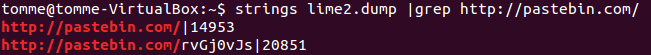
\includegraphics[scale=0.48]{strings_grep_pastebin.png}

%timeline wtf?

Finding the message, and link for the pastebin entry with \texttt{strings} and a
hex editor was not a problem, this was accomplished by a simple string search for
the string \textit{pastebin}. We were also able to find the data using Volatility's
\texttt{yarascan} plugin. The plugin allows searching by using simple strings,
or with more complex rules. For unknown reasons Volatility was not able to find
the list of running processes of this memory dump, and it had to search through 
the whole memory dump for finding the entry instead of reducing the search space 
by specific PID. 
  
\subsection{Standard Text Message}
In the third experiment we sent a text message to the standard messages application.
This was done by using the emulators’ telnet interface, where one can send a message
using the form: \texttt{sms send <phoneNumber> <textMessage>}. After sending the
message, a dump of the memory was taken. We wanted to see if it was possible to 
see recently received messages from the memory dump. Since we already knew the 
contents of the message, it was a simple matter of locating it in the memory 
dump using previous mentioned tools to do a text search. In the output of the
\texttt{yarascan} plugin we could also see the time, and phone number that was
used to send the message.
  
\subsection{Secure application - TextSecure}
Next we repeated the same experiment as above, but using the TextSecure
\footnote{\url{https://play.google.com/store/apps/details?id=org.thoughtcrime.securesms}}, 
messaging application, which encrypts messages on the disk and over the wire.
TextSecure was chosen since it is a commonly used application for securing your 
text messages in transit (both sender and receiver would need to have it 
installed) and it is open source so we could get a better understanding on 
how it manages the keys and data in memory.  
In some cases the device might have used anti-forensic tools to hide their 
activity, we wanted to look into what information a memory analysis could 
retrieve. In this experiment we were not able to retrieve any data of the message 
data.
\begin{wrapfigure}{r}{0.5\textwidth}
    \begin{center}
        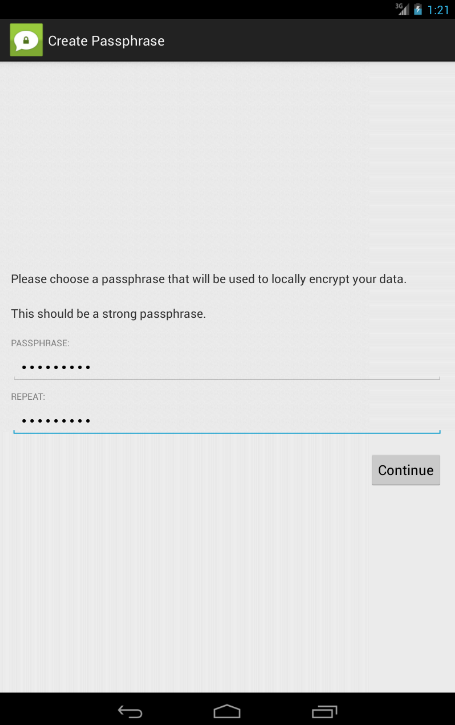
\includegraphics[scale=0.40]{textsecure.png}
    \end{center}
\end{wrapfigure}

\subsection{Screen lock}
We also did a memory dump after creating a screen lock with a PIN code and using a passphrase.
  \paragraph{Strings}
  Strings would show a lot of results since there are often many hits on readable 
  data in these kind of dumps, by piping the output to grep we were able to 
  filter out text we wanted. Simply by searching for the passphrase using grep we were able to 
  find the passphrase.

There is also a Volatility plugin created to get the PIN or passphrase from the
memory dump (\texttt{dalvik\_password}),  %??
But we had no success using this plugin.

If the device has a unlocked bootloader it would often be possible to use our 
method to retrieve memory of a device without wiping off all data from the 
device. This experiment was done to see if we could find a passphrase or 
pincode from the memory dump. By searching for the pincode and passphrase we saw a pattern,
see figure a and b. \\


\begin{figure}
        
        \begin{subfigure}[b]{0.3\textwidth}
                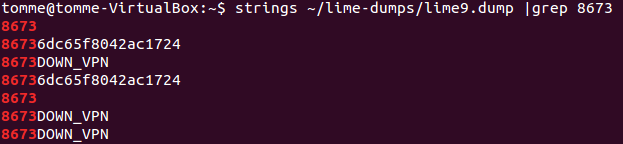
\includegraphics[scale=0.48]{strings_grep_pin.png}
                \caption{Image showing the output of strings piped into grep
                which is looking for the pin.}
                \label{fig:gull}
        \end{subfigure}%
        \qquad \qquad \qquad \qquad \qquad %add desired spacing between images, e. g. ~, \quad, \qquad, \hfill etc.
          %(or a blank line to force the subfigure onto a new line)
        \begin{subfigure}[b]{0.3\textwidth}
                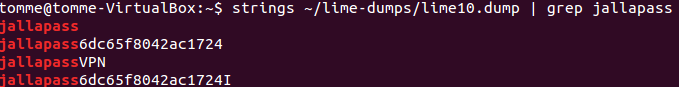
\includegraphics[scale=0.48]{strings_grep_pass.png}
                \caption{This image shows the same, but searching for a
                password instead, notice what seems to be half of a hash appended
            to the password and pin in both images.}
                \label{fig:tiger}
        \end{subfigure}
        \vspace{-20pt}

\end{figure}


\section{Discussion}
In our project we where forced to discuss some issues for the project to be % Forced?? :P
possible in our time frame. Our choice would need to be in a forensic sound manner 
so they could be applicable in a court. 

\subsection{Real phone vs. emulator}
In a real case scenario, a forensic investigator would receive a physical device 
that the investigator should acquire evidence from. However in this project there 
are a number of reasons for why we did not use a physical device.\\

While many companies give instructions on how to unlock their bootloader, they also 
state that the warranty is voided. However law-regulations in many European countries 
have better consumer laws that give the consumer rights if the fault %mangel, norsk ord
is not related to ROM or kernel of the device. Although we therefore would not have 
any real risk of loosing our rights to the producer we choose not to use our own 
devices since there always is some risk involved where the device could be bricked 
and consumer laws would not be applicable.\\

When conducting scientific experiments, it is important to do something that is 
reproducible. By using a emulator we can document how it is set up so others can 
copy the environment and get the same results. Physical devices could be a issue 
where the device is out of production.

\subsection{Secure application - TextSecure}
One of our experiments was to look into how an application that gives the user higher 
privacy by encrypting its messages. TextSecure also enables encrypted point-to-
point encryption by use of PKI. As our results have shown we did not see the 
message in the memory dump such as we did when tested against the stock SMS application. 
However, it might be possible to extract the encryption keys where the database was 
acquired and decrypt the messages. Since TextSecure is open source it is
possible to look through it's code and see how it works. We know that at some
point they have used a memory cleaner to clean sensitive memory after it has
been used.
\footnote{\url{http://goo.gl/mgDKpO}} 
The memory cleaner class was in use in the version of TextSecure we tested, so
this may be why we did not find the messages in memory. We are unsure if the
key is available in memory, as a key derivation algorithm is in use to
generate a more suitable key from the user made password. For this last
problem Volatility could have been used if we had a working version of the
Dalvik plugins in time. Then we could have made a plugin that leverages the
plugin that finds the loaded classes, and found where in the relevant
TextSecure class the keys are stored. This might require that TextSecure is
open on the device, or else the memory cleaner might overwrite the keys.

\subsection{Issues during the project}
Under the project we had some obstacles, we got a good start with researching and 
reading existing papers on the subject. However after we had decided on what 
direction we would take the project there where multiple issues when building the 
prerequisites for the kernel and emulator. There was some confusion from the guide 
on Volatility page on what to follow. Since the guide mentioned OS X specifically 
we did not pay close enough attention to what we would have to deviate from it.
%Emulator, volatility, plugins, building kernel.

\subsection{Method}
As stated earlier in the report we had a number of methods we could approach 
obtaining memory from mobile devices. When choosing method we where looking for one 
that gave us the most forensic sound evidence. Originally our chosen method was 
using \textit{pmemsave} %kommando, formatering
that was mentioned in a earlier paper\cite{acq_vol_android_mem}. However this did 
not work in the emulator, so the next best approach was chosen, where research suggests 
it gives 99.46\% identical memory dumps\cite{acq_vol_android_mem}.

\subsection{Applicable in forensic investigation}
When doing research on acquiring evidence it is important to see how it correlates 
to the real world. If the research is highly theoretical and not applicable it 
could be seen as useless. Here we discuss our thoughts on what would be different 
from a forensic investigation and our experiments.

\subsubsection{Kernel Module}
As explained in earlier chapters the LiME kernel module has to be compiled to the 
running kernel. The kernel also has to support loading of kernel modules. This is 
by default not allowed since it is a security vulnerability. This might be a 
problem if the device is running a stock ROM, where it would be necessary to obtain 
the kernel source from the producer of the device. These are often not released for 
every device and could be a issue when getting evidence in the field. Since time is 
a issue when dealing with such volatile evidence it could be feasible to have 
pre-compiled kernels and modules that would work on most common devices. However 
this might be known by the criminals. %Finnes det noe research på mobiler brukt av kriminelle? statistikk :P

\section{Conclusion}
\subsection{Real phone vs. emulator}
Warranty, guide, repreducable


\subsection{Method}

\section{Further Work}
Through this project we have been looking at what can be found in cleartext in 
the memory of android phones to get an idea of how the volatile memory in 
android devices  can be useful. Based on our findings we can say that there are
valuable information in the memory that can become relevant in a forensics case. 
From this there are a number of areas that can be researched.

The first and most critical area to make this valuable would be looking into how 
to actually get the memory of a live device, using the technique we have with 
the emulator, in most cases require a reboot of the device causing a lot of 
volatile memory to be lost.

Another topic for further work would be in developing tools to look through the 
memory data automatically, as in most cases you don't know exactly what you will 
be looking for some looking for some sort of pattern to find data consistently. 
This gets increasingly important as the memory in these devices is increasing 
quickly. Going for our test devices 800MB to newer devices 3GB of memory looking 
through this by hand is no longer realistic.

The fact that our research into secure applications isn't entirely conclusive, we
couldn't find the encryption  key or any messages sent or received using this 
secure application, but they key should probably be in the memory somehow so how 
securely hashed or stored this is might be despite the fact its not in clear text 
isn't currently known. Using a different technique and a deeper search might 
reveal different results.  

Lastly, and this is a topic we intended to research further in our own paper is 
how long different sorts of information stays in memory. This is probably 
something that will be hard to test using an emulator as actual live devices will 
have a lot more apps and background services running. And you won't be likely to 
get as clean a memory as we did with our emulator tests. 


\nocite{*}

%% The Appendices part is started with the command \appendix;
%% appendix sections are then done as normal sections
%% \appendix

%% \section{}
%% \label{}

%% References
%%
%% Following citation commands can be used in the body text:
%% Usage of \cite is as follows:
%%   \cite{key}         ==>>  [#]
%%   \cite[chap. 2]{key} ==>> [#, chap. 2]
%%

%% References with BibTeX database:

\bibliographystyle{IEEEtran}
% argument is your BibTeX string definitions and bibliography database(s)
\bibliography{IEEEabrv,bib}

%% Authors are advised to use a BibTeX database file for their reference list.
%% The provided style file elsarticle-num.bst formats references in the required Procedia style

%% For references without a BibTeX database:

% \begin{thebibliography}{00}

%% \bibitem must have the following form:
%%   \bibitem{key}...
%%

% \bibitem{}

% \end{thebibliography}

\section{Appendix 1}

\subsection{linux\_pstree output}\label{pstree}
Shortened output from the \textit{linux\_pstree} Volatility plugin.

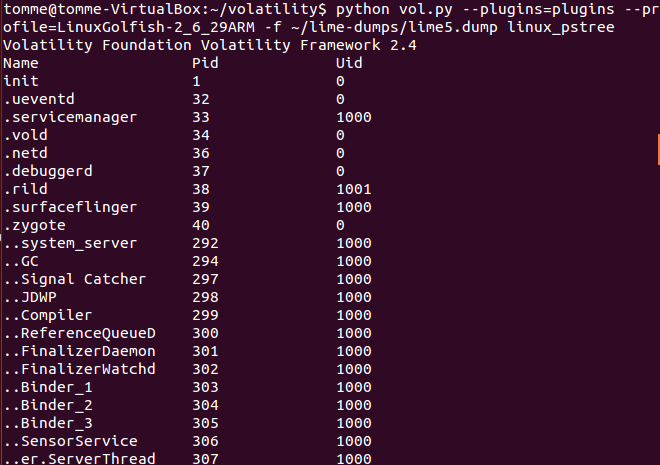
\includegraphics[scale=0.5]{linux_pstree.png}


\subsection{linux\_proc\_maps output}\label{procmaps}
Shortened output from the \textit{linux\_proc\_maps} Volatility plugin, for the
TextSecure plugin.

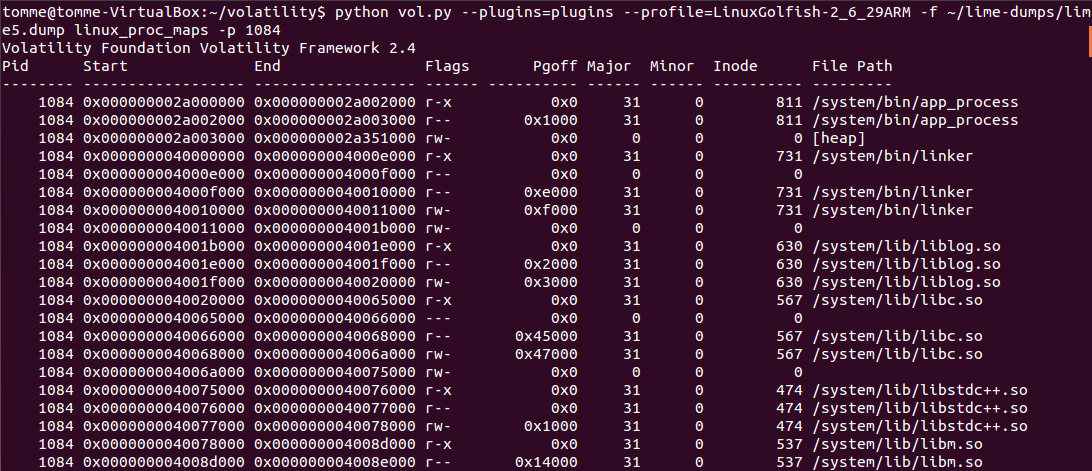
\includegraphics[scale=0.5]{linux_proc_maps.png}

\newcommand*\justify{%
  \fontdimen2\font=0.4em% interword space
  \fontdimen3\font=0.2em% interword stretch
  \fontdimen4\font=0.1em% interword shrink
  \fontdimen7\font=0.1em% extra space
  \hyphenchar\font=`\-% allowing hyphenation
}

\section{Appendix 1}
\subsection{Guide to dumping memory from Android emulator}
  This guide is based on the guide provided by Volatility \footnote{\url{https://github.com/volatilityfoundation/volatility/wiki/Android}} 
  with more detail and minor modifications.\\
  
  Get the SDK\\
  \texttt{\justify \justify wget https://dl.google.com/android/adt/adt-bundle-linux-x86\_64-20140702.zip} \\
  Unzip SDK\\
  \texttt{\justify unzip adt-bundle-linux-x86\_64-20140702.zip} \\
  Move to better path\\
  \texttt{\justify mv adt-bundle-linux-x86\_64-20140702.zip ~/android-sdk} \\
  To be able to run 32-bit on 64-bit\\
  \texttt{\justify sudo apt-get install libc6-i386 lib32stdc++6} \\
  Move to better path\\
  \texttt{\justify mv android-ndk-r10c ~/android-ndk} \\
  Install required packages\\
  \texttt{\justify sudo apt-get install openjdk-7-jdk bison g++-multilib git gperf libxml2-utils curl} \\
  Set up caache\\
  \texttt{\justify export USE\_CCACHE=1}
  Set ~/bin in your \$PATH
  \texttt{\justify mkdir ~/bin} \\
  \texttt{\justify PATH=~/bin:\$PATH} \\
  Download the repo tool and make it executable\\
  \texttt{\justify curl https://storage.googleapis.com/git-repo-downloads/repo > ~/bin/repo} \\
  \texttt{\justify chmod a+x ~/bin/repo} \\
  Create repo dir\\
  \texttt{\justify mkdir ~/android-repo \&\& cd ~/android-repo} \\
  Set git git config if you have not done so already\\
  \texttt{\justify git config --global user.email "you@example.com"} \\
  \texttt{\justify git config --global user.name "Your Name"} \\
  Initialize repo\\
  \texttt{\justify repo init -u https://android.googlesource.com/\\platform/manifest} \\
  Sync repo (this will take a long time and take up approximately 31 GB)\\
  \texttt{\justify repo sync} \\
  set up envirolment\\
  \texttt{\justify . build/envsetup.sh} \\
  Set som variables\\
  \texttt{\justify lunch full-eng} \\
  Update the SDK\\
  \texttt{\justify android update sdk -u} \\
  Before creating the AVD, you need the Image for the target we are using (4.2 API Level 17).\\
  \texttt{\justify android sdk} \\
  Select "ARM EABI v7a System Image" under API 17 and Install\\
  Create avd\\
  \texttt{\justify android avd} \\
  Set AVD name to "myavd", Device to Nexus 7 (2012) and Target to 4.2 (API Level 17). Select "Display skin with hardware controls". 
  Make sure to set the SD-card size to larger than the amount of RAM, beacuse we are saving RAM to SD-card. 
  We set 2 GB. Select Use host GPU.\\
  
  Download the Kernel source\\
  \texttt{\justify git clone https://android.googlesource.com/kernel/goldfish.git ~/android-source} \\
  \texttt{\justify cd ~/android-source/} \\
  Change branch to android-goldfish-2.6.29\\
  \texttt{\justify git checkout android-goldfish-2.6.29} \\
  Before Compiling the kernel we need to set som variables\\
  \texttt{\justify export ARCH=arm} \\
  \texttt{\justify eexport SUBARCH=arm} \\
  \texttt{\justify export CROSS\_COMPILE=arm-eabi-} \\
  Create the config file\\
  \texttt{\justify make goldfish\_armv7\_defconfig} \\
  Open the config file, and make sure the following is set:\\
  \texttt{\justify CONFIG\_MODULES=y\\ CONFIG\_MODULES\_UNLOAD=y\\ CONFIG\_MODULES\_FORCE\_UNLOAD=y\\ } \\
  Build the kernel. (when asked questions, just press enter for the default)\\
  \texttt{\justify make} \\
  You can now start the emulator\\
  \texttt{\justify emulator -avd myavd -kernel ~/android-source/arch/arm/boot/zImage -show-kernel -verbose} \\
  Download LiME\\
  \texttt{\justify git clone https://github.com/504ensicsLabs/LiME.git ~/LiME} \\
  \texttt{\justify cd ~/LiME/src} \\
  Edit the Makefile to correspond to this diff:\\
  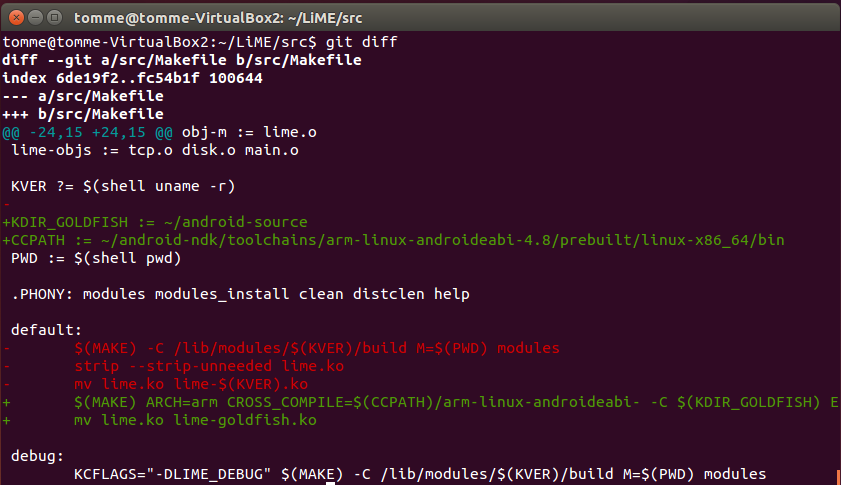
\includegraphics[scale=0.3]{diff.png} \\
  Make the kernel module\\
  \texttt{\justify make} \\
  Push the kernel module to the emulator\\
  \texttt{\justify ~/android-sdk/sdk/platform-tools/adb push ~/LiME/lime-goldfish.ko /sdcard/lime.ko} \\
  Start up a shell on the emulator\\
  \texttt{\justify ~/android-sdk/sdk/platform-tools/adb shell} \\
  In the shell type:\\
  \texttt{\justify insmod /sdcard/lime.ko "path=/sdcard/lime.dump format=lime"} \\
  You now have your memory dump in /sdcard/lime.dump\\
  Transfer it yo your PC and you you can analyse it with volatility or other tools.
  
  

\end{document}

%%
%% End of file `ecrc-template.tex'. 
